\documentclass{standalone}
\usepackage{tikz}
\usepackage{ctex,siunitx}
\usepackage{tkz-euclide}
\usepackage{amsmath}
\usetikzlibrary{patterns, calc}
\usetikzlibrary {decorations.pathmorphing, decorations.pathreplacing, decorations.shapes,}
\begin{document}
\small
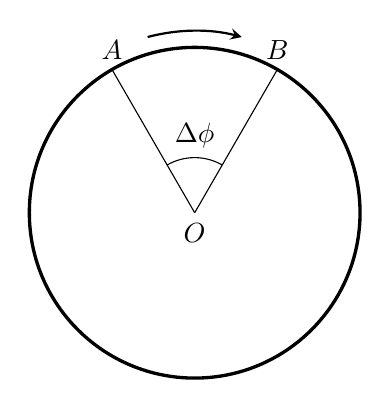
\begin{tikzpicture}[>=stealth, scale=0.7]
  \draw [very thick](0,0) node [below]{$O$} circle [radius=3];
\draw (0:0)--(60:3)node [above]{$B$};
\draw (0:0)--(120:3)node [above]{$A$};
\draw (60:1) arc (60:120:1)node [midway,above]{$\Delta \phi$};
\draw [->, thick](105:3.3) arc (105:75:3.3);
\end{tikzpicture}
\end{document}